%!TEX root = ../article/Journal_SelfCalibration.tex

\section{Appendix}
\label{sec:appendix}

Compared to the work of Grizou et al. \cite{grizou2014interactive}, we introduce a prior information on the Error-related potential EEG signals used, namely that the signal corresponding to an ``incorrect'' meaning are more ``powerful'' than the one associated to meaning ``correct''. In this appendix, we detail how we can exploit the difference of power between positive and negative ErrP signals; and show results from simulated experiments.

\subsection{Difference of power between correct and incorrect signals}

As shown in Figure~\ref{fig:EEGsample}, the EEG signals associated to ``incorrect'' labels have slightly more amplitude than the one associated to ``correct'' labels, especially around 300ms. To compute the power information contained in our signal we compute the sum of the square of each feature representing our signal. This simple approximation allows to capture the slight difference in power between ``incorrect'' and ``correct'' signals (see Figure~\ref{fig:EEGpower}). However this information alone is not enough to classify Errp signals with more than 60 percent accuracy. But considering a groups of signals we observe that the mean of power of the ``incorrect'' class is higher that the mean power of the ``correct'' class. We will exploit this property as an a priori information of which group of signal should means ``correct'' or ``incorrect''.

\begin{figure}[!htbp]
\centering
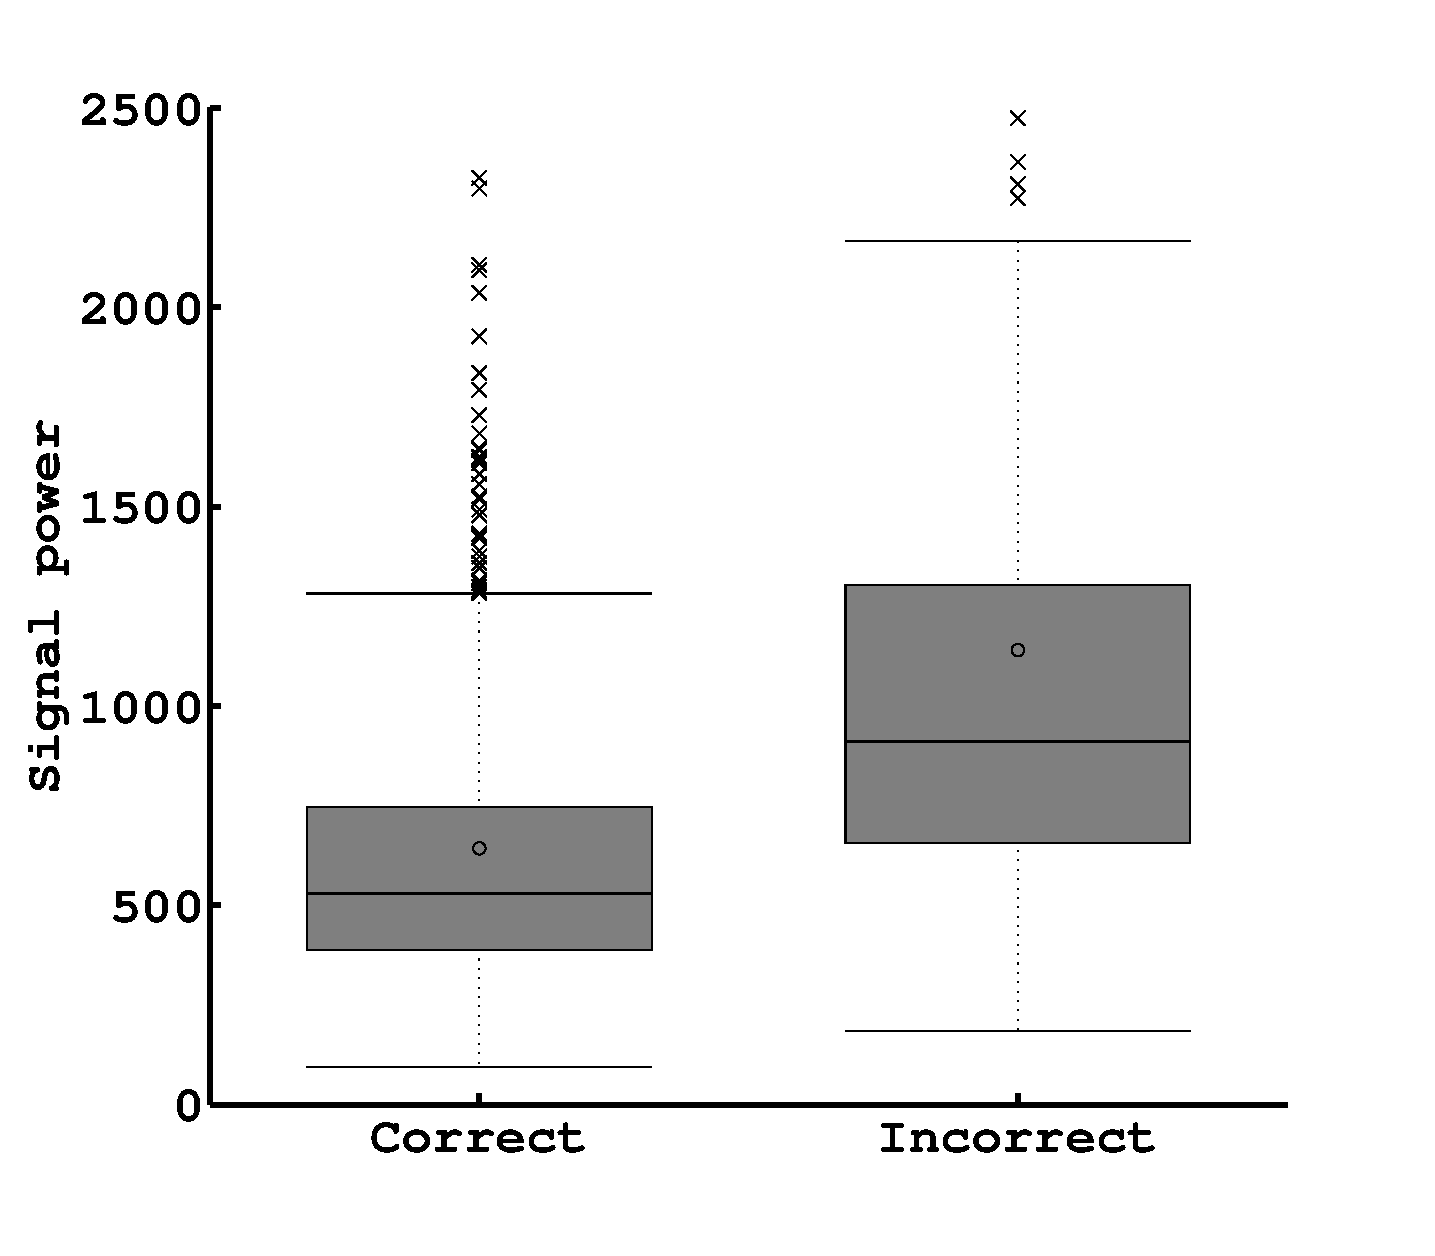
\includegraphics[width=\columnwidth]{figures/power/powerdiff.eps}
\caption{Box plot of the power of ErrP signals from one of our EEG datasets. A classifier trained on this dataset reaches a classification rate of 83 percent. The mean power information from the ``incorrect'' signals is higher than for the ``correct'' ones.}
\label{fig:EEGpower}
\end{figure} 

To compute the average power information from the signals having ``correct'' labels, we compute the weighted mean of the signals' power, with weights the probability that each signal is of label ``correct''.
\begin{eqnarray}
powerCorrect(\xi_t) = \frac{\sum_{i = 1}^{M} p(l^c = ``correct"| e_i , \theta) ~~ e_i^T e_i}{\sum_{i = 1}^{M} p(l^c = ``correct"| e_i , \theta)}
\label{eq:powerCorrect}
\end{eqnarray}
with $\theta$ representing the classifier trained on the available signal-label pairs associated to the task $\xi_t$.

Similarly, for the ``incorrect'' labels, we compute the weighted mean of the signals' power, with weights the probability that each signal is of label ``incorrect''. 
% \begin{eqnarray}
% powerIncorrect(\xi_t) = \frac{\sum_{i = 1}^{M} p(l^c = ``incorrect"| e_i , \theta) ~~ e_i^T e_i}{\sum_{i = 1}^{M} p(l^c = ``incorrect"| e_i , \theta)}
% \label{eq:powerIncorrect}
% \end{eqnarray}
% with $\theta$ representing the classifier trained on the available signal-label pairs associated to the task $\xi_t$.

\subsection{How to use the power information?}

We define a specific likelihood function for the information provided by the power information, and combine it with the information from the initial algorithm in \cite{grizou2014interactive}. We define this likelihood as the ratio of the power associated to the ``incorrect'' class over the power of the ``correct'' class:

\begin{eqnarray}
\L_{power}(\xi_t) = \frac{powerIncorrect(\xi_t)}{powerCorrect(\xi_t)}
\label{eq:power}
\end{eqnarray}

Considering the algorithm is assigning different labels for each task hypothesis, the ratio will be different for each hypothesis. The higher the ratio, the more likely the hypothesis. A symmetric interpretation of the signal will results in a negative ratio. An hypothesis whose labels are mixed will result in a ratio close to 1 because signals of low and high power will be distributed between ``correct'' and ``incorrect'' classes. 

To include this task likelihoods computed as the ratio between the power component of each class, we multiply it with the likelihood provided by the original algorithm in \cite{grizou2014interactive}. Before running online EEG experiments with human subjects, we verify how adding the power information behaves using pre-recorded datasets. 

\subsection{Comparison with and without the power information}

We consider the same grid world setting presented in section~\ref{sec:methods}, and use pre-recorder EEG signals to simulate the behavior of a subject.

\paragraph{Time to first task} Figure~\ref{fig:timefirst_powermatching} shows the number of iterations needed to reach the first target with confidence between our general method (matching), using the power information (power), or the combination of both methods (power matching). The use of the power information affects the performance for the low quality datasets (under 60 percent of accuracy). For datasets of low quality, while the time to fist target seems more advantageous when using only the power information, most of the task estimations are erroneous (see Table~\ref{tab:errorTaskRatio}), which makes the use of the power information critical for low quality data. However low quality datasets are not the main target of our algorithm. Indeed, for such data it would be better to change the representation of the brain signals or the classifier used. For datasets of higher quality (above 60 percent), the power information allows to speed up the learning compared to the initial algorithm (matching).

\begin{figure}[!htbp]
\centering
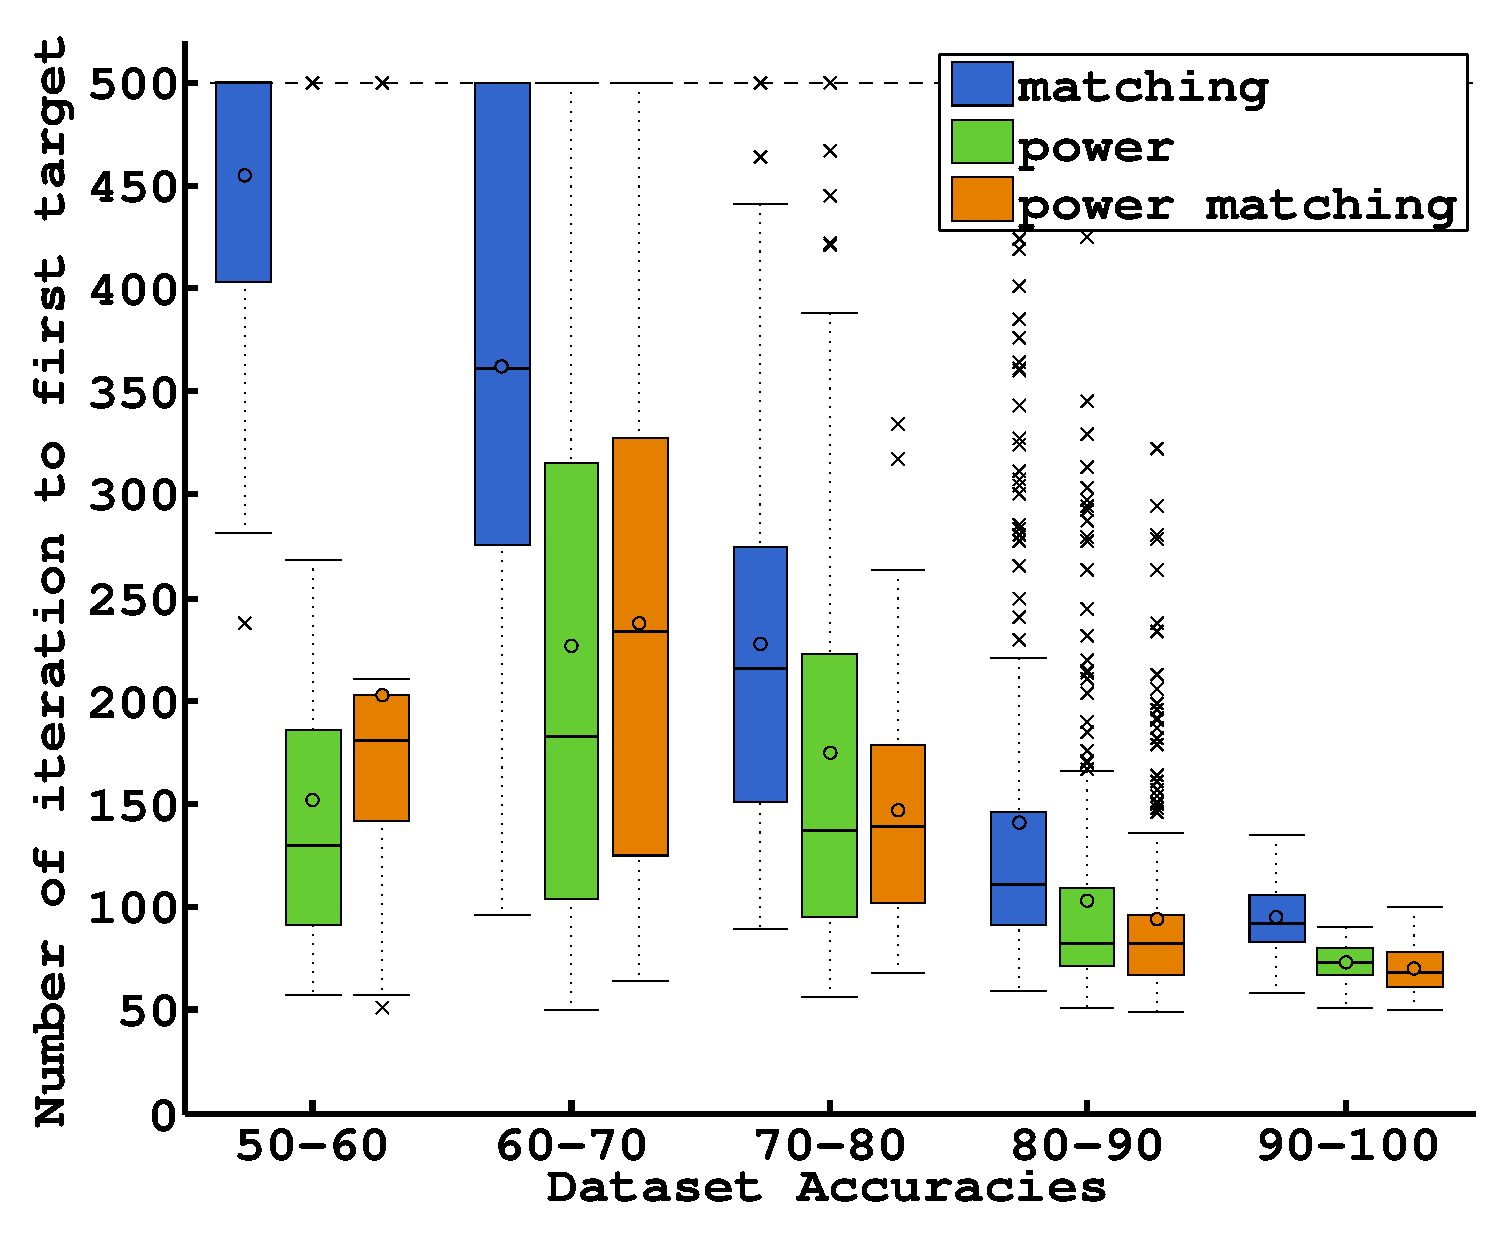
\includegraphics[width=\columnwidth]{figures/power/timefirst.eps}
\caption{Number of steps to complete the first task using EEG data. Comparison between our general method (matching), or using the information that ``incorrect'' signals are more powerful than the ``correct'' signals (power), or both methods combined (power matching). The use of the power information affects the performance for the low quality dataset (under 60 percent of accuracy).}
\label{fig:timefirst_powermatching}
\end{figure} 

\begin{table}
\centering
\rowcolors{2}{gray!25}{white}
\begin{tabular}{c c c c}
    Dataset Accuracies & Matching & Power & Power-Matching \\ \hline
    50-60 & 0 & 0.83 & 0.62 \\ 
    60-70 & 0 & 0.10 & 0.02 \\
    70-80 & 0 & 0.03 & 0.03 \\
    80-90 & 0 & 0.03 & 0.02 \\
    90-100 & 0 & 0 & 0 \\
\end{tabular}
\caption{Percentage of erroneous estimation of the first task using EEG data. Comparison between our general method (matching), or using the information that ``incorrect'' signals are more powerful than the ``correct'' signals (power), or both methods combined (power matching). For very low quality datasets (under 60 percent of accuracy), the power information increases the number of erroneous estimations.}
\label{tab:errorTaskRatio}
\end{table}

\paragraph{Number of target achieved in 500 steps}

We compare the number of target correctly (Figure~\ref{fig:nCorrect_powermatching}) and incorrectly (Figure~\ref{fig:nWrongEEG_powermatching}) completed in 500 steps between our general method (matching), using the power information (power), or both methods combined (power matching). The power information makes more mistakes for low quality dataset, which also impacts the power matching method. However these errors occur for very low quality datasets only, which are not the main target of our algorithm. For signals above 60 percent of classification rate, the power information improves the number of tasks we can reach.

\begin{figure}[!htbp]
\centering
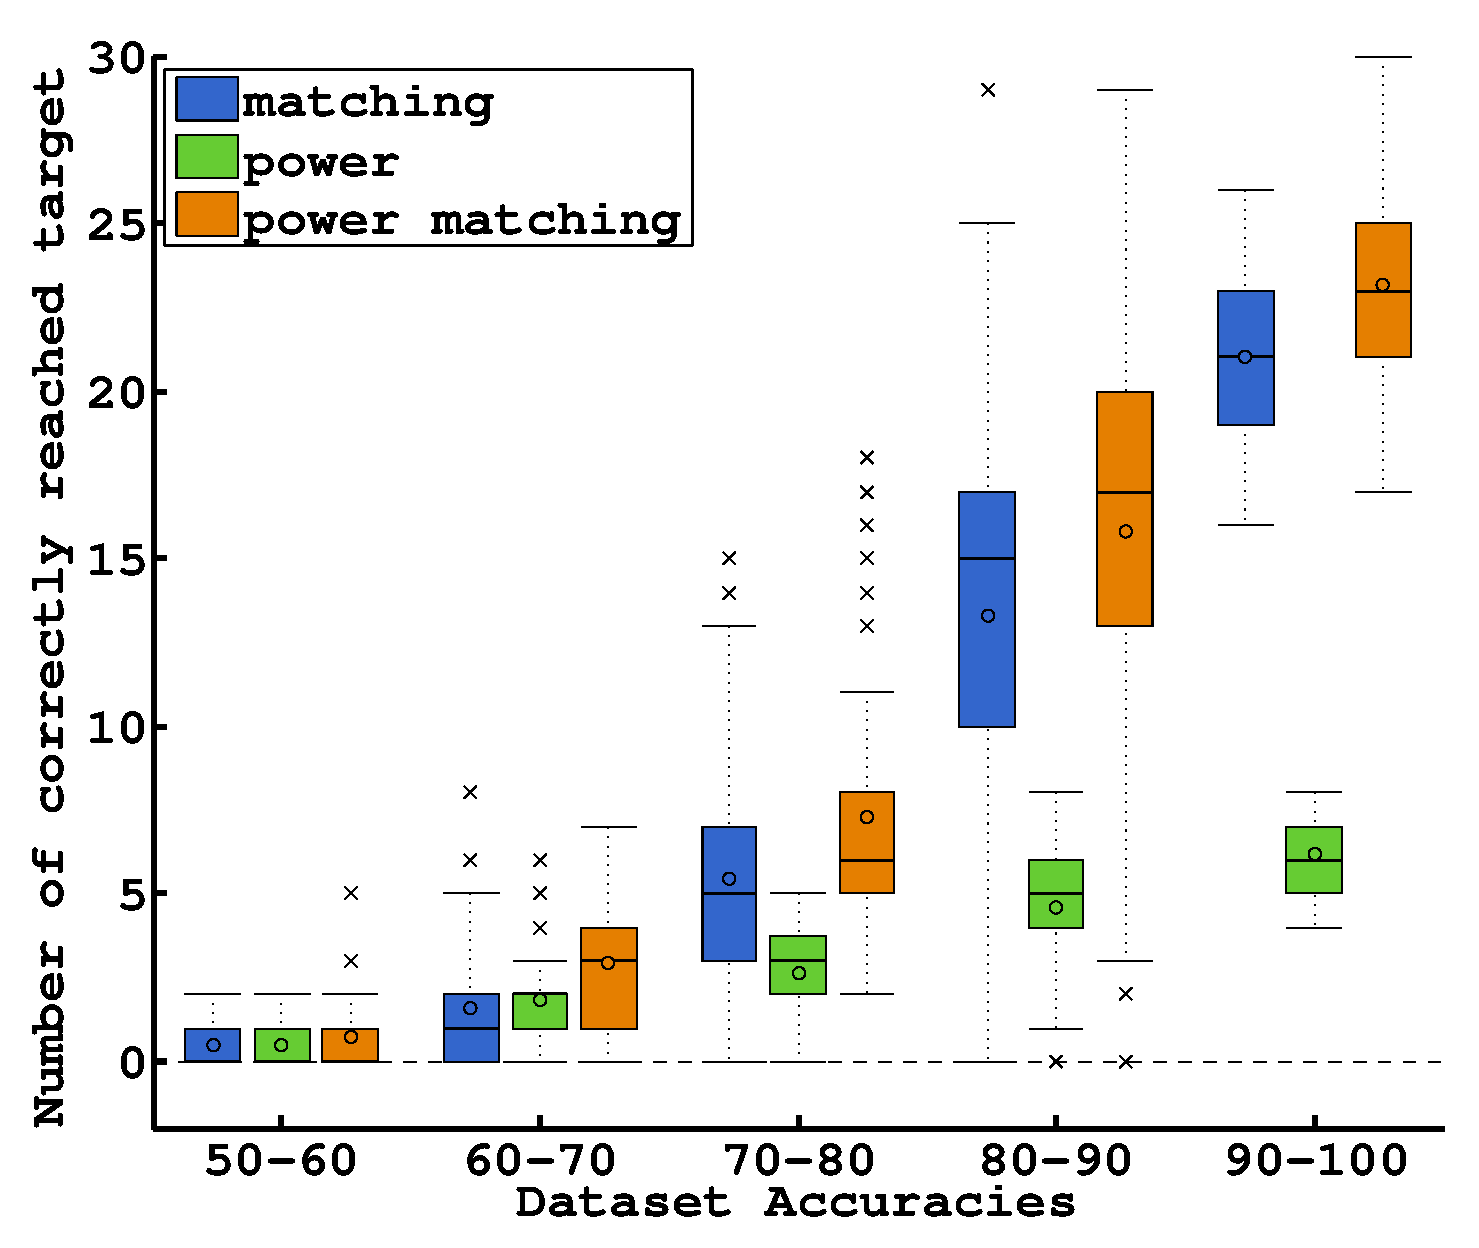
\includegraphics[width=\columnwidth]{figures/power/correct.eps}
\caption{Number of tasks correctly achieved in 500 steps with EEG data. Comparison between our general method (matching), or using the information that ``incorrect'' signals are more powerful than the ``correct'' signals (power), or both method combined (power matching). The power information alone is sufficient to solve our problem but is less efficient than the other methods.}
\label{fig:nCorrect_powermatching}
\end{figure} 

\begin{figure}[!htbp]
\centering
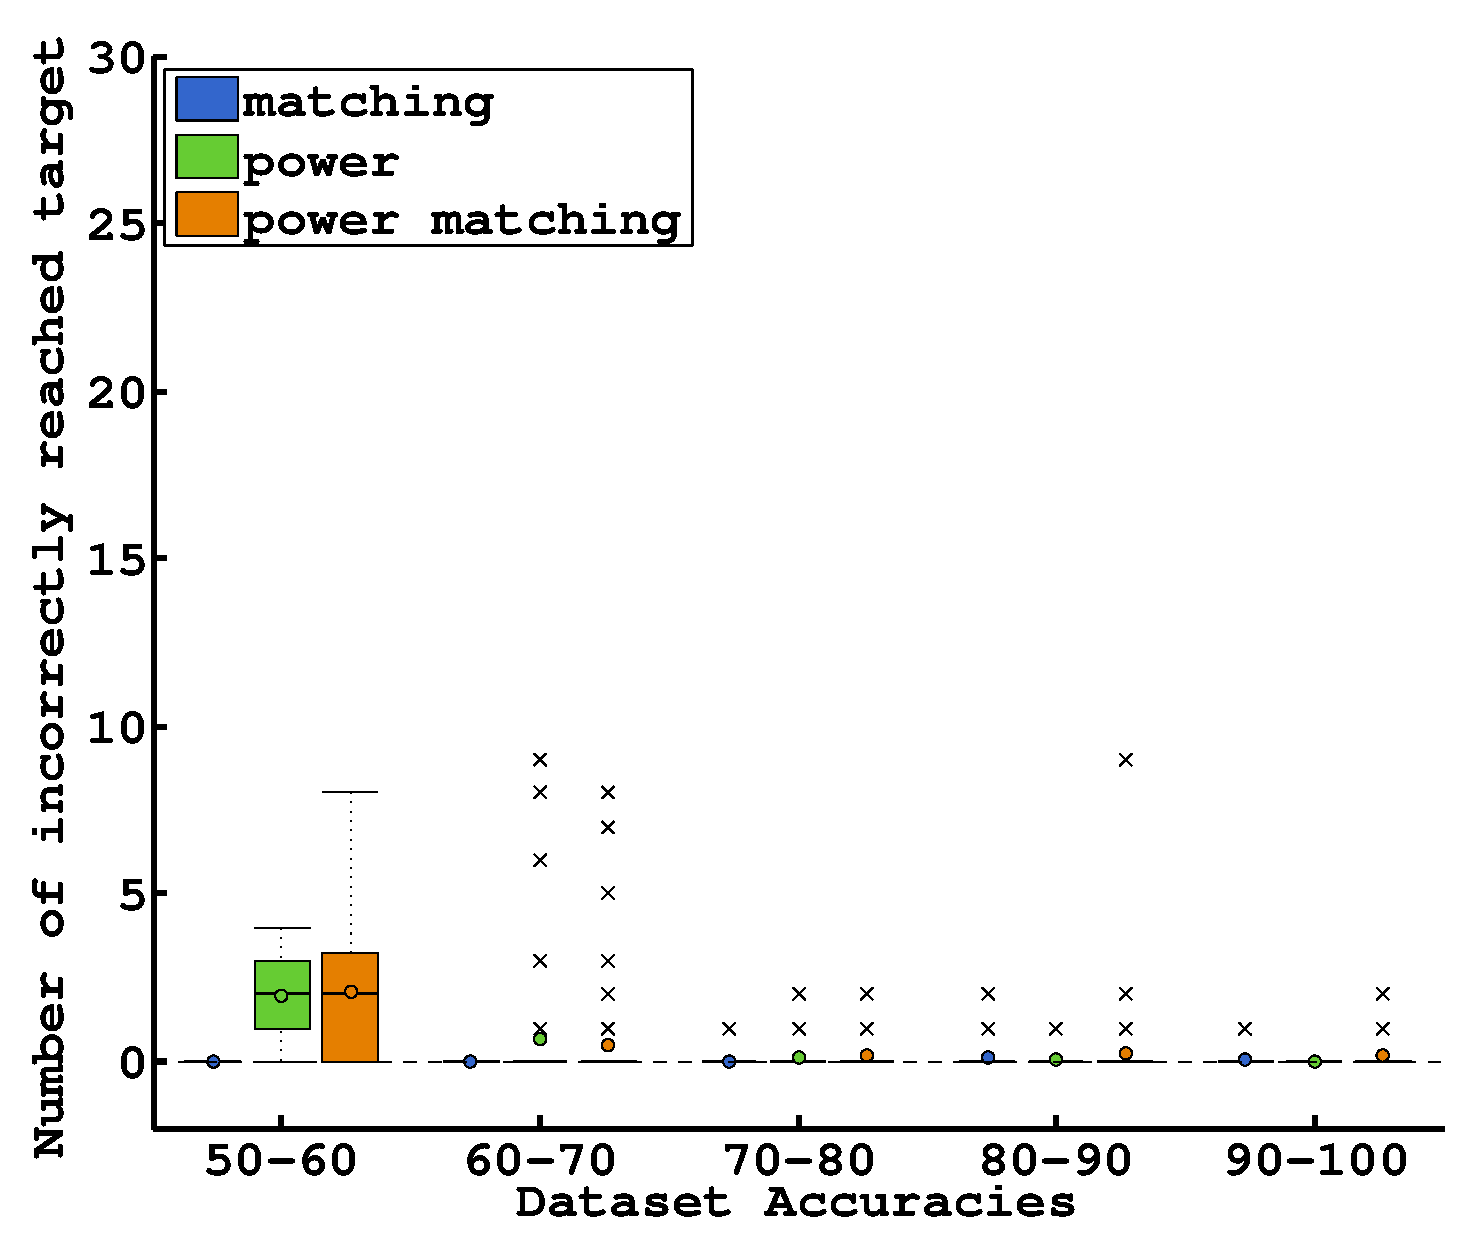
\includegraphics[width=\columnwidth]{figures/power/error.eps}
\caption{Number of tasks incorrectly achieved in 500 steps with EEG data. Comparison between our general method (matching), or using the information that ``incorrect'' signals are more powerful than the ``correct'' signals (power), or both method combined (power matching). The power information makes more mistakes for low quality dataset, which also impacts the power matching method. However these errors occur for very low quality datasets only, which are not the main target of our algorithm.}
\label{fig:nWrongEEG_powermatching}
\end{figure}

The power information alone is not enough to identify a high number of tasks, even if the number of steps to reach the first target is similar. The difference lies in the reallocation of labels, we performed after a task is identified. As described in chapter~\ref{sec:methods}, once one task is identified with confidence, we propagate its labels to all other hypotheses. As a consequence, the number of new signals with different labels needed to pull apart two hypothesis in terms of power ratio increases. This problem arises because the power information is a global measure, which depends on averaged values over all collected observations.

The results presented in this section confirm that the use of the power information improves the performance and robustness of our algorithm.
